\section{Canais Contínuos}
\begin{frame}[allowframebreaks]
  \frametitle{Canais Contínuos}
  \begin{itemize}
  \item Foi visto até o momento apenas canais discretos, modelados pela distribuição 
	de probabilidade condicional $p(y|x)$.
  \item De forma geral os canais de comunicação são contínuos e os sinais reais.
	O que ocorre em verdade é que, dada uma v.a. $X$, teremos $Y = Z(X)$,
	onde $Z$ é uma função aleatória que pode depender ou não de $X$.
  \item Isto é difícil de se analisar, portanto iremos considerar um modelo
	mais simples: ruído aditivo onde $Y = X + Z$, sendo $Z$ uma v.a..
  \item Podemos simplificar ainda mais assumindo $Z \independent X$.
  \item Podemos considerar $Z$ Gaussiano.
  \end{itemize}
\end{frame}


\subsection{Canal Gaussiano}
\begin{frame}[allowframebreaks]
  \frametitle{Canal Gaussiano}

  \begin{figure}[h!]
  \centering
  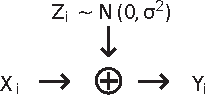
\includegraphics[width=0.3\textwidth]{images/channeladdnoisemodel.pdf}
  \label{fig:channeladdnoisemodel}
  \end{figure}

  \begin{itemize}
  \item Modelo em que $Y_i = X_i + Z_i$ com $Z_i \sim \mathcal{N} (0, \sigma^2)$ e $Z_i \independent X_i$.
  \item Quando $\sigma^2=0$ teremos um canal com capacidade infinita, pois será possível enviar um número
	real qualquer com precisão, o que pode requerer um número infinito de bits (obs: na codificação aritmética
	utilizamos uma sequência de bits tão longa quanto necessária para codificar um número no intervalo $[0,1)$).
  \item Se $\sigma^2 > 0$ podemos ter capacidade ainda infinita, pois poderemos aumentar a potência do sinal, tornando
	o ruído insignificante.
  \item Iremos tratar do problema mais realístico, quando a potência é limitada.
  \end{itemize}
\end{frame}

\begin{frame}[allowframebreaks]
  \frametitle{Limitação de Potência}
  \begin{itemize}
  \item Restrição média sobre a potência: para qualquer palavra de comprimento $n$, 
	vamos impor a seguinte restrição:
	\begin{equation}
	\frac{1}{n} \sum_{i=1}^{n} x_i^2 \leq P
	\end{equation} 
	onde $P$ é a potência média $\approx \E X^2$.
  \item Outras restrições também são possíveis, por exemplo:
	limitar o valor máximo; limitar o valor máximo em uma determinada janela.
  \end{itemize}
\end{frame}

\begin{frame}[allowframebreaks]
  \frametitle{Exemplo}
  \begin{itemize}
  \item Enviar 1 bit por vez através do canal.
  \item $X \in \{ - \sqrt{P} , + \sqrt{P} \}$, desta forma, $\E X^2 = P$, satisfazendo a restrição.
  \item Para $X$ com uma distribuição uniforme iremos decodificar como $+ \sqrt{P}$ quando $Y>0$ e 
	como $- \sqrt{P}$ quando $Y < 0$.
  \item Erro:
	\begin{eqnarray}
	P_e &=& \Pr(Y < 0 \mid X = +\sqrt{P}) \Pr(X = +\sqrt{P}) + \nonumber \\
		&& \Pr(Y > 0 \mid X = -\sqrt{P}) \Pr(X = -\sqrt{P}) \\
	    &=& \Pr(Z < -\sqrt{P} \mid X = +\sqrt{P}) \frac{1}{2} + \Pr(Z > +\sqrt{P} \mid X = -\sqrt{P}) \frac{1}{2} \\
		&& \text{como } Z \independent X \nonumber \\
	    &=& \Pr(Z > \sqrt{P})
	\end{eqnarray}
  \item $Z$ possui distribuição Gaussiana. Os dois tipos de erro (quando $Y < 0 \mid X = +\sqrt{P}$ e $Y > 0 \mid X = -\sqrt{P}$) 
	são ilustrados abaixo.

  \begin{figure}[h!]
  \centering
  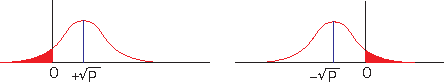
\includegraphics[width=0.6\textwidth]{images/gausschanexerror.pdf}
  \label{fig:gausschanexerror}
  \end{figure}


  \item Erro total ($\times 1/2$):

  \begin{figure}[h!]
  \centering
  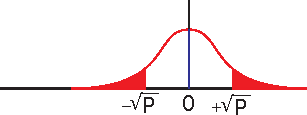
\includegraphics[width=0.5\textwidth]{images/gausschanexerror2.pdf}
  \label{fig:gausschanexerror2}
  \end{figure}

  \item Teremos assim
	\begin{equation}
	\Pr(Z > \sqrt{P}) = 1 - \Phi \left( \frac{\sqrt{P}}{\sigma^2} \right)
	\end{equation}
	onde $\Phi$ é a distribuição normal cumulativa, i.e.,
	\begin{equation}
	\Phi (x) = \int_{-\infty}^{x} \frac{1}{\sqrt{2 \pi}} e^{-t^2 / 2} dt
	\end{equation}

  \item Desta forma, transformamos um canal Gaussiano em um canal binário simétrico onde $p = P_e$.

  \begin{figure}[h!]
  \centering
  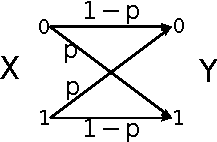
\includegraphics[width=0.33\textwidth]{images/bsch.pdf}
  \label{fig:bsch111}
  \end{figure}

  \item Podemos converter um canal contínuo em um canal discreto, utilizando uma codificação
	apropriada para tanto.
 
  \item Este é um processo de quantização vetorial. Para cada esquema de quantização devemos analisar
	a relação de compromisso entre a taxa e a distorção sob determinada restrição de potência.

  \begin{figure}[h!]
  \centering
  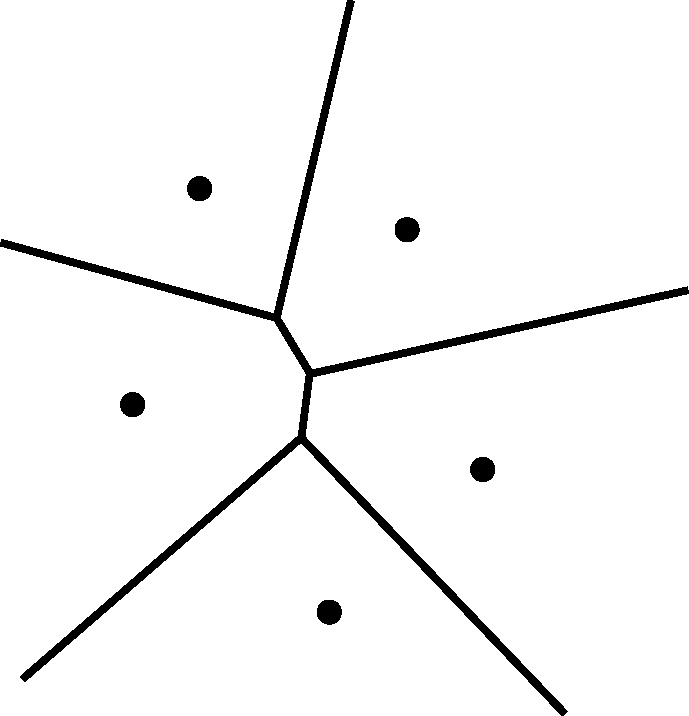
\includegraphics[width=0.33\textwidth]{images/voronoi.pdf}
  \label{fig:voronoi}
  \end{figure}

  \end{itemize}
\end{frame}


\begin{frame}[allowframebreaks]
  \frametitle{Capacidade do Canal Gaussiano}

  \begin{definition}
  A capacidade (de informação com restrição de potência $P$) é definida como
	\begin{equation}
	C = \max_{p(x): \E X^2 \leq P} I(X;Y) \text{bits}
	\end{equation}
  \end{definition}

  \begin{itemize}
  \item Aqui foi dada apenas a definição, nada foi dito com relação à possibilidade de comunicar 
	a uma taxa igual, menor ou maior a esta capacidade.
  \item $I(X;Y)$ será da seguinte forma
	\begin{eqnarray}
	I(X;Y) &=& h(Y) - h(Y|X) = h(Y) - h(X + Z | X) \\
		&=& h(Y) - h(Z|X) = h(Y) - h(Z)
	\end{eqnarray}
  \item Note que, quando $X \independent Z$, teremos $h(X+Z) \geq h(Z)$, e desta forma teremos $I(X;Y) \geq 0$.
  \item Estratégia para encontrar $C$: 1) limitar $I(X;Y)$; 2) encontrar $p(x)$ (não necessariamente única)
	que alcança o limite.
  \item $Z$ é Gaussiana, logo $h(Z) = \frac{1}{2} \log (2 \pi e \sigma^2)$ onde $\sigma^2$ é a potência do ruído,
	$\E Z^2 = \sigma^2 = N$, com $\E Z = 0$.
  \item Vimos anteriormente que a entropia de uma Gaussiana é limitada pelo segundo momento da seguinte forma,
	considerando $\E X = 0$ e $\Var X = K$,
	\begin{equation}
	h(X) \leq \frac{1}{2} \log [(2 \pi e)^2 | K |]
	\end{equation}
  \item Teremos também
	\begin{eqnarray}
	\E Y^2 &=& \E (X+Z)^2 = \E X^2 + \underbrace{2 \E X \E Z}_{\text{pois } X \independent Z} + \E Z^2 \\
		&=& \underbrace{P}_{\text{potência do sinal,} \E X^2} + \underbrace{\sigma^2}_{\text{potência do ruído,} \E Z^2}
	\end{eqnarray}
  \item Podemos limitar a informação mútua, utilizando o limite para a entropia de uma Gaussiana.
	\begin{eqnarray}
	I(X;Y) &=& h(Y) - h(Z) \leq \frac{1}{2} \log (2 \pi e (P+\sigma^2)) - \frac{1}{2} \log (2 \pi e \sigma^2) \nonumber \\
		&=& \frac{1}{2} \log \left( 1 + \frac{P}{\sigma^2} \right) = \frac{1}{2} \log (1 + \text{SNR})
	\end{eqnarray}
	onde SNR é a relação sinal-ruído.
  \item Como visto anteriormente, a Gaussiana possui entropia máxima dentre todas as distribuições que possuem 
	os mesmos momentos de primeira e segunda ordem.
  \item Poderemos alcançar a informação mútua máxima se garantirmos que $Y$ é gaussiano, ou seja,
	como $Z$ \textit{a priori} gaussiano, devemos escolher $X$ gaussiano, pois a soma de gaussianas 
	é gaussiana, e assim garantiremos que $Y$ é gaussiano.
  \item Desta forma, a capacidade de um canal Gaussiano é
	\begin{equation}
	C = \frac{1}{2} \log \left( 1 + \frac{P}{\sigma^2} \right) = \frac{1}{2} \log (1 + \text{SNR})
	\end{equation}
  \item A capacidade será alcançada quando $X \sim \mathcal{N}(0,P)$.
  \end{itemize}
\end{frame}


\begin{frame}[allowframebreaks]
  \frametitle{Exemplo: PCM 6dB SNR/bit}

  \begin{itemize}
  \item Dado um sinal limitado em frequência $x(t)$ tal que $X(f) = 0$ para $f > f_c$,
	se amostrarmos este sinal a uma taxa $1/\tau \geq 2 f_c$ (taxa de Shannon/Nyquist),
	teremos reconstrução perfeita.
	\begin{equation}
	x[n] = x(n \tau)
	\end{equation}
	onde $\tau$ é o período de amostragem.
  \item Cada uma das amostras é quantizada e representada por um inteiro.

  \begin{figure}[h!]
  \centering
  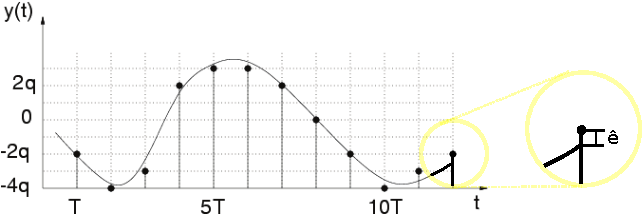
\includegraphics[width=0.75\textwidth]{images/sampling.pdf}
  \label{fig:sampling}
  \end{figure}

  \item A quantização pode ser modelada por um canal gaussiano, i.e.,
	\begin{equation}
	\hat{x}[n] = x[n] + \eta_n = x(n\tau) + \eta_n
	\end{equation}
	onde $\hat{x}[n] = jq$ para um inteiro $q \in \mathbb{Z}$, $q$ é o quantum (passo) de quantização
	e $\eta_n \sim \mathcal{N}(0,\sigma^2)$ é um ruído gaussiano aditivo.
  \item Utilizando $b$ bits para representar cada valor quantizado, teremos no máximo $2^b$ valores 
	possíveis diferentes para $\hat{x}[n]$.
  \item Utilizando a equação obtida para a capacidade de uma canal Gaussiano
        \begin{equation}
        C = \frac{1}{2} \log \left( 1 + \frac{P}{\sigma^2} \right) = \frac{1}{2} \log (1 + \text{SNR})
        \end{equation}
  \item Para 6dB que aumentamos a SNR, será necessário $\frac{1}{2} \log (1 + 2)$ bits a mais na capacidade 
	do canal.
  \item Tipicamente, para áudio, temos $b=16$ bits e, desta forma, SNR de 96 dB.
  \item Teremos assim
	\begin{equation}
	16 \text{bits/utilização do canal} = \frac{1}{2} \log (1 + \text{SNR})
	\end{equation}
	desta forma, $2^{32} = 1 + \text{SNR}$ e assim $\text{SNR} = 2^{32} - 1$.
  \item Em escala logaritmica
	\begin{equation}
	10 \log_{10} (\text{SNR}) \approx 10 \times 32 \log_{10} 2 \approx 96.33 \text{dB}
	\end{equation}
	e assim teremos $96.33/16 \approx 6.02 \text{dB/bit}$.
  \item Cada bit adicional em um áudio PCM adiciona $6.02$ dB na SNR.
  \end{itemize}
\end{frame}


\begin{frame}[allowframebreaks]
  \frametitle{Capacidade de Canal}

  \begin{definition}[código]
  Um código $(M,n)$ para um canal Gaussiano, com restrição de potência $P$, inclui
  \begin{enumerate}
  \item conjunto de índices $\{1, 2, \ldots, M\}$
  \item função de codificação $X: \{1, 2, \ldots, M\} \rightarrow \mathcal{X}^n$, fornecendo
	palavras $X^n(1), X^n(2), \ldots, X^n(M)$ tais que
	\begin{equation}
	\frac{1}{n} \sum_{i=1}^{n} X_i^2(\omega) \leq P, \quad \forall \omega \in \{1, \ldots, M\}
	\end{equation}
  \item função de decodificação
	\begin{equation}
	g: \mathcal{Y}^n \rightarrow \{1, \ldots, M\}
	\end{equation}
  \end{enumerate}
  \end{definition}

  \framebreak

  \begin{definition}[taxa]
  A taxa é dada por
	\begin{equation}
	R = \frac{\log M}{n} \text{bits por utilização do canal}
	\end{equation}
  \end{definition}

  \begin{definition}[taxa alcançável]
  Um taxa $R$ é alcançável se $\exists$ uma sequência de códigos $(2^{nR},n)$ satisfazendo a
  restrição de potência $P$ tal que $\lambda^{(n)} \rightarrow 0$ (a probabilidade máxima de erro) 
  quando $n \rightarrow \infty$.
  \end{definition}

  \begin{definition}[capacidade]
  A capacidade de um canal Gaussiano é o supremo de todas as taxas alcançáveis
  (i.e., o maior valor possível alcançável).
  \end{definition}

  \framebreak

  \begin{theorem}[Capacidade do canal Gaussiano]
  A capacidade de um canal Gaussianoo com restrição $P$ na potência de entrada e ruído 
  com variância $\sigma^2$ é dada por
	\begin{equation}
	C = \frac{1}{2} \log \left( 1 + \frac{P}{\sigma^2} \right) \text{bits por utilização do canal}
	\end{equation}
  \end{theorem}

  \begin{proof}
  \begin{itemize}
  \item O conjunto típico em $X$, $A_{\epsilon}^{(n)}$, possui volume $\leq 2^{n(h(X) + \epsilon)}$.
  \item O conjunto condicionalmente típico em $Y$ possui volume $\leq 2^{n(h(Y|X) + \epsilon)} = 2^{n(h(Z) + \epsilon)}$.
  \item O conjunto típico em $Y$ (incondicional) possui volume $\leq 2^{n(h(Y) + \epsilon)}$, mas
	temos que $h(Y) \leq \frac{1}{2} \log [2 \pi e (P + \sigma^2)]$ e $h(Z) = \frac{1}{2} \log [ 2 \pi e \sigma^2 ]$.
  \end{itemize}
  \proofbreak
  \begin{itemize}
  \item Quantos volumes condicionais em $X$ podemos empacotar dentro do volume total?
	\begin{equation}
	\leq \frac{2^{nh(Y)}}{2^{nh(Z)}} = \frac{2^{n \frac{1}{2} \log [2 \pi e (P+\sigma^2)]}}{2^{n\frac{1}{2} \log [2 \pi e \sigma^2]}} \approx 2^{\frac{n}{2} \log \frac{P+\sigma^2}{\sigma^2}} = [(P+\sigma^2)/\sigma^2]^{n/2}
	\end{equation}
  \item Iremos assumir o melhor cenário (taxa máxima), sem sobreposição dos volumes.
  \item Teremos
	\begin{equation}
	2^{nR} = 2^{\frac{n}{2} \log \frac{P + \sigma^2}{\sigma^2}} \text{ e assim, } R = \frac{1}{2} \log (1 + P/\sigma^2)
	\end{equation}
  \end{itemize}
  \proofbreak
  \begin{itemize}
  \item Se tudo for conjuntamente Gaussiano i.i.d., os volumes típicos serão esferas.
  \item Volume da esfera (em $n$-D)
	\begin{equation}
	V(r,n) = \frac{\pi^{n/2}}{\Gamma \left( \frac{n}{2} + 1 \right)} r^n = 2^{\frac{n}{2} \log [2 \pi e \sigma^2]} = (2\pi e r^2)^{n/2}
	\end{equation}
	teremos assim
	\begin{equation}
	r_{\sigma^2} = \Gamma^{1/2} \left( \frac{n}{2} + 1 \right) (2 e \sigma^2)^{1/2}
	\end{equation}
  \end{itemize}

  \proofbreak

  \begin{itemize}
  \item Quantas esferas pequenas cabem dentro da esfera maior?

	\begin{figure}[h!]
	\centering
	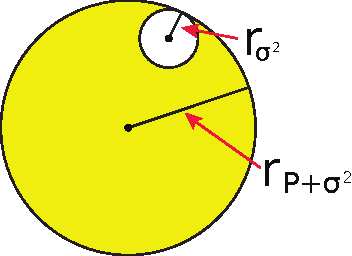
\includegraphics[width=0.4\textwidth]{images/spherepack.pdf}
	\label{fig:spherepack}
	\end{figure}

  \item Semelhente ao que foi feito no caso discreto (a razão entre os volumes fornece o limite).
  \end{itemize}

  \proofbreak

  \begin{itemize}
  \item Precisamos mostrar que se $R < C$, $\exists$ um código com $P_e^n \rightarrow 0$ quando $n \rightarrow \infty$.
  \item Geramos palavras de código aleatórias (assim como feito no caso discreto), mas neste caso
	com Gaussianas com $\E X^2 = P - \epsilon$, de forma que
	\begin{equation}
	\frac{1}{n} \sum_{i=1}^{n} x_i^2 \rightarrow P - \epsilon \text{ quando } n \rightarrow \infty
	\end{equation}
  \end{itemize}
  \proofbreak

  \begin{itemize}
  \item Teremos uma fonte adicional de erro possível (quando não for satisfeita a restrição em potência)
	\begin{equation}
	E_0 = \left\{ \frac{1}{n} \sum_{i=1}^{n} x_i^2(1) > P \right\}
	\end{equation}
  \item Devemos adicionar $E_0$ aos demais erros vistos anteriormente no caso discreto.
  \item Pela lei fraca dos grandes números, $E_0 \rightarrow 0$ quando $n \rightarrow \infty$ assim como
	para as demais fontes de erro.
  \end{itemize}

  \end{proof}
\end{frame}


\begin{frame}[allowframebreaks]
  \frametitle{Limitação em Banda}
  \begin{itemize}
  \item Suponha que o canal seja limitado em frequência, ou seja, $H(j\omega) = 0$ para $\vert \omega \vert > W$,
	onde $W$ é a largura de banda do canal, $\omega$ é a variável que representa frequência e $H(j\omega)$
	é a resposta em frequência do canal, ou seja, transformada de Fourier de $h(t)$ (resposta ao impulso).
  \item Podemos ver a saída como
	\begin{equation}
	Y(t) = (X(t) + Z(t)) \ast h(t)
	\end{equation}
	desta forma, se o canal for limitado em frequência, teremos um sistema não-causal,
	ele agirá como enviando a saída através de um filtro passa-baixas antes de observá-la.
  \item Resposta ao impulso de um filtro limitado em banda.
	\begin{equation}
	h(t) \xleftrightarrow{\text{FT}} H(j\omega)
	\end{equation}
  \item Como esta restrição irá influenciar a capacidade?
  \item Se o sinal é limitado em banda com limite $W$, quantas amostras por segundo serão necessárias?
	$2W$ amostras por segundo, de forma que teremos uma amostra a cada $\tau = 1/2W$ segundos.
  \item Grosseiramente, se um sinal é `aproximadamente' limitado em frequência ($W$) e no tempo ($T$),
	podemos descrever o sinal apropriadamente com $2WT$ coeficientes/amostra.
  \item Dado um sinal $x(t)$ aproximadamente limitado em tempo e frequência, utilizando uma base apropriada
	(por exemplo, senoides truncadas de comprimento $T$), a representação
	\begin{equation}
	x(t) = \sum_{i=-WT}^{WT} \alpha_i \psi_i(t) + x_r(t)
	\end{equation}
	terá erro residual pequeno, i.e., $\Vert x_r(t) \Vert$ é pequeno quando utilizarmos $2WT$
	coeficientes $\{\alpha_i\}_i$.
  \item Modelo do ruido aditivo.
        \begin{figure}[h!]
        \centering
        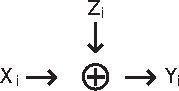
\includegraphics[width=0.3\textwidth]{images/channeladdnoisemodel2.pdf}
        \label{fig:channeladdnoisemodel2}
        \end{figure}
  \item Vamos assumir que o ruído possui densidade espectral de potência $\sigma^2/2$ watts/hertz e
	largura de banda de $W$ hertz, então a potência do ruído é $\frac{\sigma^2}{2} 2W = \sigma^2 W$.
  \item A energia total é $\sigma^2 WT$ (potência = energia por unidade de tempo ou, neste caso, por amostra).
  \item Cada amostra possui variância:
	 energia total / número de amostras $= \sigma^2 WT/(2WT) = \sigma^2/2$.
  \item $Z = Y|X$ possui distribuição da forma
	\begin{equation}
	Y|X \sim \mathcal{N} \left( 0, \frac{\sigma^2}{2} I \right)
	\end{equation}
  \item Isto pode ser visto como uma esfera típica no espaço de recepção.
  \item A potência do sinal por amostra da entrada dada por: energia total / número de amostras $= TP/2WT = P/2W$.
  \item A potência do ruído por amostra da saída é $\sigma^2/2$.
  \item Utilizando esses valores na fórmula da capacidade em função da SNR $=$ potência
	do sinal por amostra / variância do ruído por amostra, teremos
	\begin{equation}
	C = \frac{1}{2} \log \left( 1 + \frac{P/2W}{\sigma^2/2} \right) = \frac{1}{2} \log \left( 1 + \frac{P}{\sigma^2W} \right) 
	\text{bits/amostra}
	\end{equation}
  \item Como existem $2W$ amostras por segundo, teremos
	\begin{equation}
	C = W \log \left( 1 + \frac{P}{\sigma^2W} \right) \text{bits por segundo}
        \end{equation}
  \item Podemos aumentar a capacidade: 1) aumentando a largura de banda $W$; 2) aumentando a potência do sinal $P$ ou;
	3) reduzindo a variância do ruído $\sigma^2$.
  \end{itemize}
  \framebreak
  \begin{itemize}
  \item Gráfico de $C$ em função de $W$ para $\sigma^2$ fixo.
        \begin{figure}[h!]
        \centering
        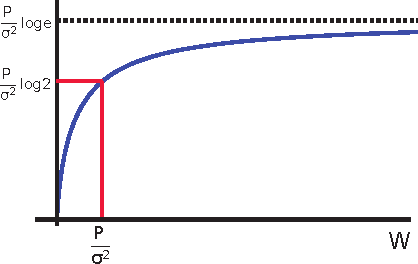
\includegraphics[width=0.6\textwidth]{images/capchannelband.pdf}
        \label{fig:capchannelband}
        \end{figure}

  \item Observamos que $C$ cresce rápidamente quando $W \in [0, P/\sigma^2]$ e a partir deste ponto
	$C$ cresce mais devagar com $C_\infty = \left( \frac{P}{\sigma^2} \right) \log e$.
  \end{itemize}

  \begin{exercise}[Linha Telefônica]
  Para permitir a multiplexação de diversos canais em uma linha telefônica,
  o sinal telefônico é limitado a uma banda com largura de 3300 Hz. Supondo que a linha
  telefônica esteja sujeita a ruído e que a relação sinal-ruído máxima da linha
  é de 33 dB, encontre a capacidade do canal telefônico em bits por segundos.
  (Os modems reais atingem uma taxa de transmissão de até 33.600 bits por segundo.
  Em linhas telefônicas reais outros fatores influenciam a capacidade do canal como,
  por exemplo, interferências, linhas cruzadas, ecos, e característica não-plana
  do canal telefônico.
  \exercisebreak 
  Os modems V.90 atingiam 56 kb/s em apenas uma direção utilizando o canal telefônico,
  tirando proveito da linha digital pura entre o servidor e a central telefônica final da rede.
  Nesta caso, os únicos empecilhos são devidos a conversão analógico-digital na central e
  o ruído no link de cobre da central até a residência: estes empecilhos reduzem a taxa de bits
  máxima de 64 kb/s do sinal digital na rede para 56 kb/s nas melhores linhas telefônicas.
  A largura de banda efetiva do fio de cobre é da ordem de alguns megahertz; o que depende
  do comprimento da linha. A resposta em frequência também não é plana. Se toda a largura de banda
  for utilizada, é possível enviar alguns megabits por segundo através do canal; o que é o
  caso do DSL (Digital Subscriber Line).
  \exercisebreak
  \textit{(solução)}
  Vamos utilizar $10^{3.3} \approx 2000$ e $\log_2 1000 = 9.9658$.
  O ruído possui densidade de potência espectral $N_0/2$ watts/hertz e largura de banda $W$.
  A potência do ruído é $\frac{N_0}{2} 2W = N_0 W$.
  \begin{eqnarray}
  C &=& W \log \left( 1 + \frac{P}{N_0 W} \right) \\
  &=& W \log \left( 1 + \text{SNR} \right) = 3300 \log (1 + 10^{3.3}) \\
  &=& 3300 \log \left( 2000 \right) = 3300 (\log 2 + \log 1000) \\
  &=& 3300 \times (1 + 9.9658) \\
  &=& 36187 \text{ bits / s}
  \end{eqnarray}
 
  \end{exercise}
\end{frame}



\subsection{Canais em Paralelo}
\begin{frame}[allowframebreaks]
  \frametitle{Canais em Paralelo}
  \begin{itemize}
  \item Sejam $k$ canais em paralelo.
  \end{itemize}

        \begin{figure}[h!]
        \centering
        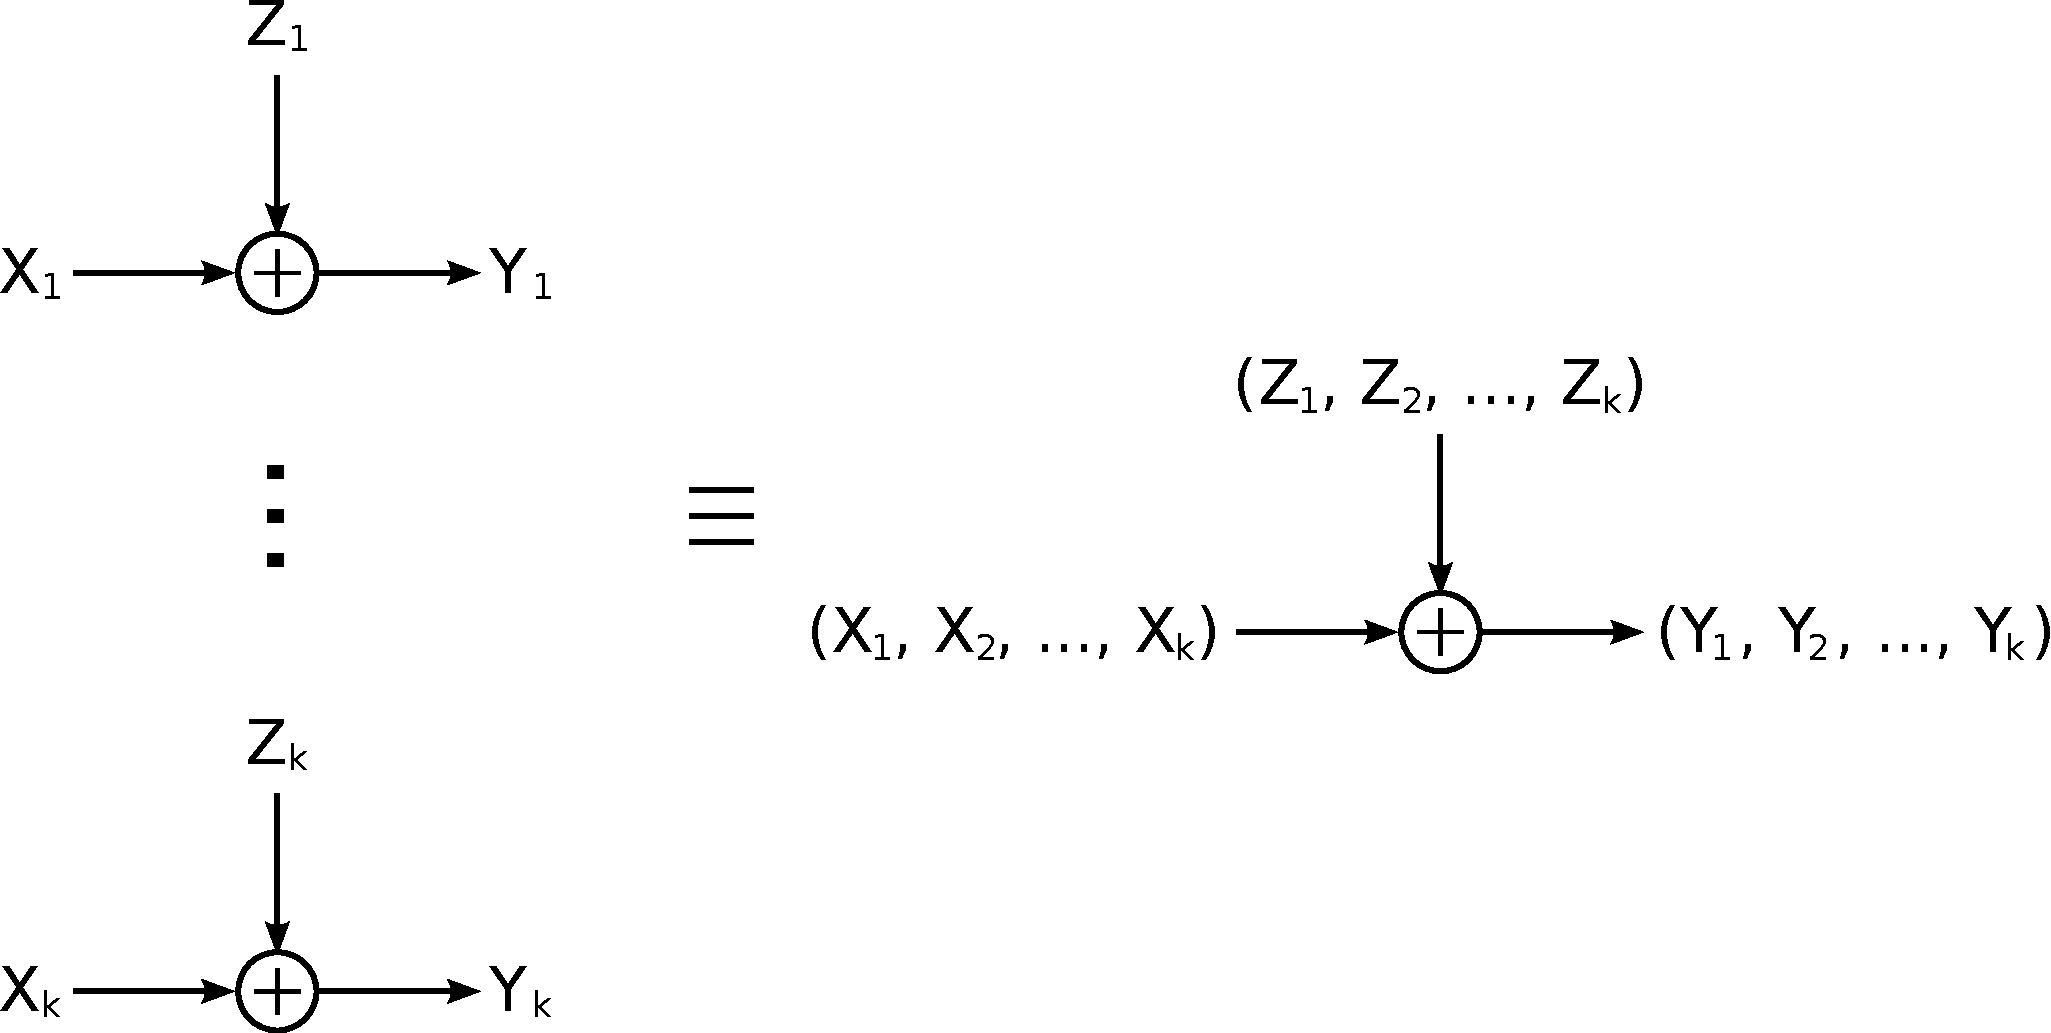
\includegraphics[width=0.7\textwidth]{images/parallelchannels.pdf}
        \label{fig:parallelchannels}
        \end{figure}

  \begin{itemize}
  \item O ruido é caracterizado por
	\begin{equation}
	\begin{pmatrix}
	Z_1 \\ Z_2 \\ \vdots \\ Z_k
	\end{pmatrix} \sim
	\mathcal{N} \left(0, 
		\begin{bmatrix} N_1 & 0 & \ldots & & 0 \\
				0 & N_2 & 0 & \ldots & 0 \\
				\vdots & & \ddots &  & \vdots \\
				0 & \ldots & & 0 & N_k 
		\end{bmatrix}
	  \right)
	\end{equation}
  \item Os ruídos não são correlacionados já que $Z_i \independent Z_j$ para $i \neq j$.

  \item Sem restrições, a capacidade será $C = \log \left( \sum_i 2^{C_i} \right)$, se utilizarmos
	um canal por vez, e será $\sum_i C_i$, se utilizarmos simultâneamente.
  \item Qual será a capacidade se houve uma restrição comum de potência?
	\begin{equation}
	\E \left[ \sum_{j=1}^{k} X^2_j \right] = \sum_{j=1}^{k} \E X_j = \sum_i P_i \leq P
	\end{equation}

        \begin{figure}[h!]
        \centering
        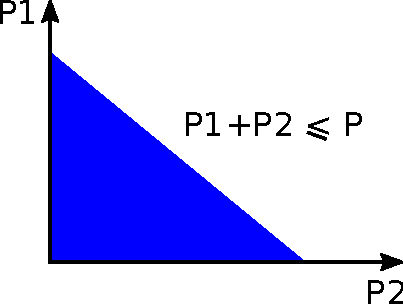
\includegraphics[width=0.3\textwidth]{images/pconstraint.pdf}
        \label{fig:pconstraint}
        \end{figure}

  \item Objetivo agora é encontrar a capacidade, dada a restrição de potência.
	\begin{equation}
	C = \max_{f(x_{1:k}) : \sum_i \E X_i^2 \leq P} I(X_{1:k}; Y_{1:k})
        \end{equation}

  \item Teremos o seguinte
	\begin{eqnarray}
	I(X_{1:k}; Y_{1:k}) &=& h(Y_{1:k}) - h(Y_{1:k} | X_{1:k}) = h(Y_{1:k}) - h(Z_{1:k} | X_{1:k}) \nonumber \\
		&=& h(Y_{1:k}) - h(Z_{1:k}) = h(Y_{1:k}) - \sum_{j=1}^{k} h(Z_{j}) \\
		&\leq& \sum_{j} \left( h(Y_{j}) - h(Z_{j}) \right) \leq \sum_{j} C_j = \sum_{j} \frac{1}{2} \log \left( 1 + \frac{P_i}{N_i} \right) \nonumber
	\end{eqnarray}
	onde $P_i = \E X_i^2$ e $\sum_i P_i = P$.

  \item A igualdade ocorrerá quando
        \begin{equation}
        \begin{pmatrix}
        X_1 \\ X_2 \\ \vdots \\ X_k
        \end{pmatrix} \sim
        \mathcal{N} \left(0, 
                \begin{bmatrix} P_1 & 0 & \ldots & & 0 \\
                                0 & P_2 & 0 & \ldots & 0 \\
                                \vdots & & \ddots &  & \vdots \\
                                0 & \ldots & & 0 & P_k 
                \end{bmatrix}
          \right)
        \end{equation}


  \item Teremos o seguinte problema de otimização para solucionar:
        \begin{equation}
        \begin{aligned}
        & \underset{(P_1, P_2, \ldots, P_n)}{\text{maximizar}}
        & & \sum_j \frac{1}{2} \log \left(1 + \frac{P_i}{N_i} \right) \\
        & \text{sujeito a} & & \sum_i P_i = P
        \end{aligned}
        \end{equation}

  \item Lagrangiano será da forma
	\begin{equation}
	J(P_{1:n}) = \sum_{j} \frac{1}{2} \left( 1 + \frac{P_i}{N_i} \right) + \lambda \left( \sum_{j} P_j - P \right)
	\end{equation}

  \end{itemize}
\end{frame} 


\begin{frame}[allowframebreaks]
  \frametitle{Otimização de Lagrange}
  \begin{itemize}
  \item Forma geral de uma problema de otimização:
	\begin{equation}
	\begin{aligned}
	& \underset{x}{\text{minimizar}}
	& & f_0(x) \\
	& \text{sujeito a}
	& & f_i(x) \leq 0, \; i = 1, \ldots, m, \\
	& & & h_i(x) = 0, \; i = 1, \ldots, p.
	\end{aligned}
	\end{equation}

  \item Forma do Lagrangiano
	\begin{equation}
	L(x, \lambda, \nu) = f_0(x) + \sum_{i=1}^{m} \lambda_i f_i (x) + \sum_{i=1}^{p} \nu_i h_i (x)
	\end{equation}
	e vamos definir
	\begin{equation}
	g(\lambda, \nu) = \inf_{x} L(x, \lambda, \nu)
	\end{equation}

  \item $g$ é côncava em $(\lambda, \nu)$, já que $g$ é o ínfimo ponto-a-ponto sob uma transformação
	afim de $(\lambda, \nu)$, i.e.,
	\begin{equation}
	f(\lambda, \nu) = \min_{x \in \{a,b\}} (f_1(x) \lambda + f_2 (x) \nu + f_c)
        \end{equation}
	será côncava.

        \begin{figure}[h!]
        \centering
        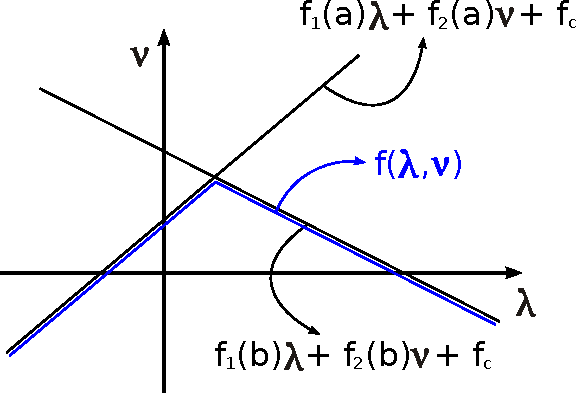
\includegraphics[width=0.5\textwidth]{images/fnulambda.pdf}
        \label{fig:fnulambda}
        \end{figure}

  \item Novamente, a definição de $L$ é
        \begin{equation}
        L(x, \lambda, \nu) = f_0(x) + \sum_{i=1}^{m} \lambda_i f_i (x) + \sum_{i=1}^{p} \nu_i h_i (x)
        \end{equation}

  \item Considerando $\lambda \geq 0$, teremos, para o ponto ótimo $x_{\text{opt}}$ (um ponto factível),
	que $\lambda_i f_i (x_{\text{opt}}) \leq 0$, como $\lambda_i \geq 0$, teremos $f_i (x_{\text{opt}}) \leq 0$,
	e $h_i (x_{\text{opt}}) = 0$.
	\begin{equation}
	\begin{aligned}
	\sum_{i=1}^{p} \nu_i h_i (x_{\text{opt}}) = 0 & \quad & \sum_{i=1}^{m} \lambda_i f_i (x_{\text{opt}}) \leq 0
	\end{aligned}
	\end{equation}
  \item Definiremos $p_{\text{opt}} = L(x_{\text{opt}}, \lambda, \nu)$ e desta forma
	\begin{equation}
	g(\lambda, \nu) = \inf_x L(x,\lambda, \nu) \leq p_{\text{opt}} = L(x_{\text{opt}}, \lambda, \nu) \leq f(x_{\text{opt}})
	\end{equation}
  \end{itemize}

\end{frame}



\begin{frame}[allowframebreaks]
  \frametitle{Exemplo de restrição severa}
  \begin{itemize}
  \item Considere a seguinte função
	\begin{equation}
	L^{\square}(x) = f_0 (x) + \sum_{i=1}^{m} \left[ \frac{1}{\mathbf{1} (f_i(x) \leq 0)} - 1 \right] 
			+ \sum_{i=1}^{p} \left[ \frac{1}{\mathbf{1} (h_i(x) = 0) } - 1 \right]
	\end{equation}
  \item Note que, quando algum das restrições é violada, teremos $L^{\square} = \infty$. Se todas as
	restrições são satisfeitas, teremos $L^{\square} (x) = f_0 (x)$.
  \item Para $\lambda_i > 0$ temos
	\begin{equation}
	\lambda_i f_i (x) \leq \left[ \frac{1}{\mathbf{1} (f_i(x) \leq 0)} - 1 \right]
	\end{equation}
	e para qualquer $\nu_i \in \mathbb{R}$, temos
	\begin{equation}
	\nu_i h_i (x) \leq \left[ \frac{1}{\mathbf{1} (h_i(x) = 0) } - 1 \right]
	\end{equation}
  \item Devemos então ter
	\begin{equation}
	L(x, \lambda, \nu) \leq L^{\square}(x) \quad \forall \lambda > 0, \nu
	\end{equation}
  \item Seja $x_{\text{opt}} = \min_x L^{\square}(x)$.
  \item Para quaisquer $\lambda > 0$ e $\nu$,
	\begin{equation}
	\inf_x L(x, \lambda, \nu) \triangleq g(\lambda, \nu) \leq L(x_{\text{opt}}, \lambda, \nu) \leq L^{\square}(x_{\text{opt}}) = f(x_{\text{opt}})
	\end{equation}
  \item O melhor (maior) limite inferior, definirá valores ótimos duais, i.e.
	\begin{equation}
	(\lambda_{\text{opt}}, \nu_{\text{opt}}) \in \argmax_{\lambda \geq 0 , \nu} g(\lambda, \nu)
	\end{equation}
  \item Definiremos $d_{\text{opt}} = g(\lambda_{\text{opt}}, \nu_{\text{opt}})$.
  \end{itemize}
\end{frame}


\begin{frame}[allowframebreaks]
  \frametitle{Dualidade fraca e intervalo de dualidade}
  \begin{itemize}
  \item A condição de dualidade fraca será dada quando o dual máximo não for
	maior do que o mínimo principal, i.e.,
	\begin{equation}
	d_{\text{opt}} \leq p_{\text{opt}} \Leftrightarrow \text{dualidade fraca}
	\end{equation}
  \item Note que a dualidade fraca será verdadeira pois, para quaisquer $x', \lambda', \nu'$ teremos
	\begin{equation}
	g(\lambda', \nu') = \inf_x L(x,\lambda', \nu') \leq L(x', \lambda', \nu') \leq 
		\sup_{\lambda > 0, \nu} L(x',\lambda, \nu) \leq L^{\square} (x')
	\end{equation}
  \item Assim,
	\begin{equation}
	d_{\text{opt}} = \sup_{\lambda > 0, \nu} L(x,\lambda, \nu) \leq \inf_x \sup_{\lambda > 0, \nu} L(x,\lambda, \nu) = \inf_x L^{\square} (x) = p_{\text{opt}}
	\end{equation}
  \item Teremos assim o seguinte intervalo de dualidade
	\begin{equation}
	p_{\text{opt}} - d_{\text{opt}} \geq 0
	\end{equation}
  \end{itemize}
\end{frame}

\begin{frame}[allowframebreaks]
  \frametitle{Dualidade forte e intervalo de dualidade nulo}
  \begin{itemize}
  \item No caso de dualidade forte, teremos $p_{\text{opt}} = d_{\text{opt}}$.
  \item Podemos seguir maximizando o dual e minimizando o primário, se os dois se encontrarem,
	saberemos que achamos o ótimo (ou se estiverem próximos, teremos um limite para a qualidade
	da solução obtida).
  \item Infelizmente a dualidade forte nem sempre é satisfeita, enquanto a dualidade fraca é sempre verdadeira.
  \item Condições de Slater (condições para que a dualidade forte seja satisfeita):
	Se $f_i$ são convexas e existem soluções que sejam estritamente factíveis 
	(i.e., $\exists x$ tal que $\forall i$, $f_i(x) < 0$ e $A_i x = b_i$, de forma que
	$h_i(x) = A_i x - b_i$), então a dualidade forte será verdadeira.
  \item O intervalo de dualidade é importante para limitar a qualidade da solução
	\begin{equation}
	f_0 (x) - p_{\text{opt}} \leq f_0 (x) - g(\lambda, \nu) \quad \forall \lambda, \nu
	\end{equation}
  \item Note que $f_0 (x) - g(\lambda, \nu)$ é o intervalo de dualidade associado entre $x$ primário
	factível e o ponto dual factível $(\lambda, \nu)$.
  \item O intervalo de dualidade pode ser utilizado como critério para para o processo de otimização.
	Se o intervalo for nulo, então atingimos o ótimo.
  \item Assumindo dualidade forte, $p_{\text{opt}} = d_{\text{opt}}$, teremos
	\begin{eqnarray}
	f_0(x_{\text{opt}}) &=& g(\lambda_{\text{opt}}, \nu_{\text{opt}}) \\
			&=& \inf_x \left( f_0(x) + \sum_{i=1}^{n} \lambda_i^\ast f_i (x) + \sum_{i=1}^{p} \nu_i^\ast h_i(x) \right) \label{eqstrgopt1} \\	
			&\leq& f_0(x_{\text{opt}}) + \sum_{i=1}^{n} \lambda_i^\ast f_i (x_{\text{opt}}) + \sum_{i=1}^{p} \nu_i^\ast h_i(x_{\text{opt}}) \label{eqstrgopt2} \\
			&\leq& f_0(x_{\text{opt}}) \label{eqstrgopt3}
	\end{eqnarray}
	onde $\lambda_{\text{opt}} = (\lambda_1^\ast , \lambda_2^\ast, \ldots)$, e  de forma similar para $\nu_{\text{opt}}$.
	\begin{itemize}
	\item \ref{eqstrgopt1} segue da definição
	\item \ref{eqstrgopt2} segue do ínfimo e dualidade fraca
	\item \ref{eqstrgopt3} segue de $\lambda_i^\ast \geq 0$, $f_i(x_{\text{opt}}) \leq 0$ e $h_i(x_{\text{opt}}) = 0$.
	\item teremos igualdade em \ref{eqstrgopt2} e \ref{eqstrgopt3} por causa da dualidade forte.
	\end{itemize}


  \item Cada um dos termos do Lagrangiano será nulo, i.e.,
	\begin{equation}
	\left[ \lambda_i^\ast f_i(x_{\text{opt}}) \leq 0, \forall i \quad \text{e} \quad 
		\sum_{i=1}^{m} \lambda_i^\ast f_i(x_{\text{opt}}) = 0 \right] \Rightarrow
		 \lambda_i^\ast f_i(x_{\text{opt}}) = 0 , \forall i
	\end{equation}
  \item Uma condição necessária para a otimalidade será 
	\begin{equation}
	\text{se} \quad \lambda_i^\ast > 0 \quad \text{então} \quad f_i(x_{\text{opt}}) = 0
	\end{equation}
	ou
	\begin{equation}
	\text{se} \quad  f_i(x_{\text{opt}}) < 0 \quad \text{então} \quad \lambda_i^\ast = 0
        \end{equation}
	uma das condições de Karush–Kuhn–Tucker (KKT) para otimalidade.
  \item Cada um dos $f_i$ será uma restrição ativa (i.e. $f_i(x_{\text{opt}}) = 0$) ou então
	serão não-ativos ($f_i(x_{\text{opt}}) \leq 0$) e assim $\lambda_i^\ast = 0$.
  \item Se todas as funções são diferenciáveis, então existe $\nabla f_0$, $\nabla f_i$
	e $\nabla h_i$.
  \item Como $p_{\text{opt}} = \min_x \max_{\lambda > 0, \nu} L(x, \lambda, \nu) = \min_x L(x, \lambda_{\text{opt}}, \nu_{\text{opt}})$ teremos
	\begin{equation}
	\nabla_x L \vert_{x = x_{\text{opt}}, \lambda = \lambda_{\text{opt}} , \nu = \nu_{\text{opt}}} = 0
	\end{equation}
  \item Então, uma outra condição para otimalidade é
	\begin{equation}
	\nabla_x f_0 (x_{\text{opt}}) + \sum_{i=1}^{m} \lambda_i^\ast \nabla_x f_i (x_{\text{opt}}) +
	\sum_{i=1}^{p} \nu_i^\ast \nabla_x h_i (x_{\text{opt}}) = 0
	\end{equation}
  \item As condições de KKT para otimalidade serão
	\begin{equation}
	f_i(x_{\text{opt}}) \leq 0 \quad \text{para} \quad i = 1, \ldots , m
	\end{equation}
        \begin{equation}
        h_i(x_{\text{opt}}) = 0 \quad \text{para} \quad i = 1, \ldots , p
        \end{equation}
        \begin{equation}
        \lambda_i^\ast \geq 0 \quad \text{para} \quad i = 1, \ldots , m
        \end{equation}
        \begin{equation}
        \lambda_i^\ast f_i(x_{\text{opt}}) = 0 \quad \text{para} \quad i = 1, \ldots , m
        \end{equation}
	e
	\begin{equation}
	\nabla_x L \vert_{x = x_{\text{opt}}, \lambda = \lambda_{\text{opt}}, \nu = \nu_{\text{opt}}} = 0
        \end{equation}
	aonde utilizamos a notação $\lambda_{\text{opt}} = \lambda^\ast$ e $\nu_{\text{opt}} = \nu^\ast$.
  \end{itemize}
\end{frame}


\begin{frame}[allowframebreaks]
  \frametitle{Canais Paralelo}
  \begin{itemize}
  \item Queremos solucionar o problema
        \begin{equation}
        \begin{aligned}
        & \underset{(P_1, P_2, \ldots, P_n)}{\text{maximizar}}
        & & \sum_j \frac{1}{2} \log \left(1 + \frac{P_i}{N_i} \right) \\
        & \text{sujeito a} & & \sum_i P_i = P
        \end{aligned}
        \end{equation}

  \item ou na forma do Lagrangiano
        \begin{equation}
        J(P_{1:n}) = \sum_{j} \frac{1}{2} \left( 1 + \frac{P_i}{N_i} \right) + \lambda \left( \sum_{j} P_j - P \right)
        \end{equation}

  \item $x = (P_1, P_2, \ldots, P_m)$ é um vetor de potências
  \item $N_i$ ruído dado em cada canal ($\sigma_i^2$)
  \item Queremos
	\begin{equation}
	\text{minimizar} \quad - \sum_{i=1}^{k} \log (1 + P_i / N_i)
        \end{equation}
	sujeito às desigualdades de restrição $P_i \geq 0$ (então $f_i (P_i) = - P_i$) e
 	igualdades de restrição $\sum_{i=1}^{k} P_i = P$ (i.e. $h = (\sum_{j=1}^n P_i - P) = 0$).
  \item Este problema é convexo.
  \item Então existe um ponto estritamente factível. Desta forma a dualidade forte é válida, assim
	como as condições de KKT para a otimizalidade.
  \end{itemize}


  \framebreak

  \begin{itemize}
  \item Teremos o seguinte Lagrangeano:
	\begin{equation}
	L(x,\lambda,\nu) = - \sum_{i=1}^{k} \log (1 + P_i / N_i) - \sum_{i=1}^k \lambda_i P_i + \nu \left( \sum_{i=1}^k P_i - P \right)
	\end{equation}

  \item As codiçoes de KKT serao:
	\begin{equation}
	\forall i : P_i^\ast \geq 0 , \quad \sum_i P_i^\ast = P , \quad \lambda_i^\ast \geq 0 \forall i, \quad \lambda_i^\ast P_i^\ast = 0
	\end{equation}
	e também, $\forall i$
	\begin{equation}
	- \frac{1}{(1 + P_i / N_i)} \frac{1}{N_i} - \lambda_i^\ast + \nu^\ast = 0
	\end{equation}
  \item A partir das condicoes do gradiente do Lagrangeano, podemos ainda obter
	\begin{equation}
	- \frac{1}{N_i + P_i} - \lambda_i^\ast + \nu^\ast = 0
	\end{equation}
	\begin{equation}
	- \frac{1}{N_i + P_i} + \nu^\ast = \lambda_i^\ast \geq 0
	\end{equation}
  \item Podemos eliminar $\lambda_i^\ast$ para obter as condiçoes de KKT na forma
	\begin{eqnarray}
	\forall i : P_i^\ast \geq 0  & \sum_i P_i^\ast = P \\
	\left( \nu^\ast - \frac{1}{N_i + P_i} \right) P_i^\ast = 0 & \nu^\ast \geq \frac{1}{N_i + P_i^\ast}
	\end{eqnarray}
  \end{itemize}

  \framebreak

  Temos entao dois casos:
  \begin{description}
  \item[Caso 1]: 
 	\begin{itemize}
	\item a partir da condiçao $\nu^\ast \geq \frac{1}{N_i + P_i^\ast}$, se $\nu^\ast < 1 / N_i$, entao
	devemos ter $P_i^\ast > 0$ para alcançar esta condiçao.
	\item Em tal caso, como temos $\left( \nu^\ast - \frac{1}{N_i + P_i} \right) P_i^\ast = 0$, devemos ter
	$\nu^\ast = \frac{1}{N_i + P_i^\ast}$.
	\item Assim, $P_i^\ast = \frac{1}{\nu^\ast} - N_i$.
	\end{itemize}
  \item[Caso 2]:
	\begin{itemize}
        \item se $\nu^\ast \geq 1/N_i$, entao $P_i^\ast = 0$, já que no caso contrário ($P_i^\ast > 0$) 
	significaria
		\begin{equation}
		\underbrace{ \left( \nu^\ast - \frac{1}{N_i + P_i} \right) }_{> 0 \text{ já que } \nu^\ast \geq 1/N_i \text{ e } P_i^\ast > 0} \times \underbrace{ P_i^\ast }_{> 0} > 0
		\end{equation}
	\end{itemize}
  \end{description}
 

  \framebreak

  \begin{itemize}
  \item $P_i^\ast$ deverá ser da forma
	\begin{eqnarray}
	P_i^\ast &=& \begin{cases}
			1/\nu^\ast - N_i & \quad \text{ se } \nu^\ast < 1 / N_i , \\
			0 		& \quad \text{ se } \nu^\ast \geq 1 / N_i .
			\end{cases}  \\
		&=& \max \{ 0, 1/\nu^\ast - N_i \}
	\end{eqnarray}
  \item com a ultima restriçao teremos
	\begin{equation}
	\sum_i \left( \frac{1}{\nu^\ast} - N_i \right)^{+} = P
	\end{equation}
	onde $a^{+} = \max \{ 0, a\}$.

  \item isto leva à ideia da água enchendo os canais em paralelo.
  \end{itemize} 

     \begin{figure}[h!]
     \centering
     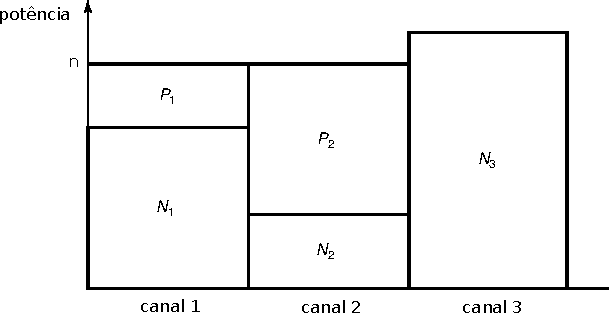
\includegraphics[width=0.75\textwidth]{images/waterfilling.pdf}
     \label{fig:waterfilling}
     \end{figure}

  \framebreak

  A capacidade final será
  \begin{eqnarray}
  C_n &=& \frac{1}{2} \sum_{j=1}^{k} \log (1 + P_i / N_i) \\
	&=& \frac{1}{2} \sum_{j=1}^{k} \log \left( 1 + \frac{(1/\nu^\ast - N_i)^{+}}{N_i} \right)
  \end{eqnarray} 
  Em unidades de bits por transmissao (bits por transmissao em canal simples, tomando a média):
  \begin{eqnarray}
  C_n &=& \frac{1}{2n} \sum_{j=1}^{k} \log \left( 1 + \frac{(1/\nu^\ast - N_i)^{+}}{N_i} \right) \text{ bits por transmissao}
  \end{eqnarray}

\end{frame}


